\chapter{Evaluation}
\label{cap:Evaluation}
This chapter will describe the evaluation, the goal is to test signatures and rules detection algorithm. First the evaluation method is presented and then the results. The last section  of this chapter is answering the research questions. 

\section{Evaluation Method}
This section describes the method used to evaluate the thesis results. The evaluation process reuse network infrastructure, capturing process and data filtering as in the original research. Some new aspects are included in the evaluation to make the environments more representative for smart environments. These new aspects are describes in detail further in this section.

\subsubsection{Evaluation environments}
Event triggering during evaluation was conducted in three different environments, now called Guestroom, Bedroom and Living room. Environment layout is shown in Figure \ref{fig:Liveroom}. The Irobot Roomba i7 was reverted to factory default for each of the evaluation environments, this mitigates the change of any interference between the environments. User input such as robot, floor and room names was configured differently for all environments. A map discovery process was executed as part of the inital set-up phase.

\begin{figure}[H]
    \centering
    
    \begin{subfigure}{0.35\textwidth}
        \centering
        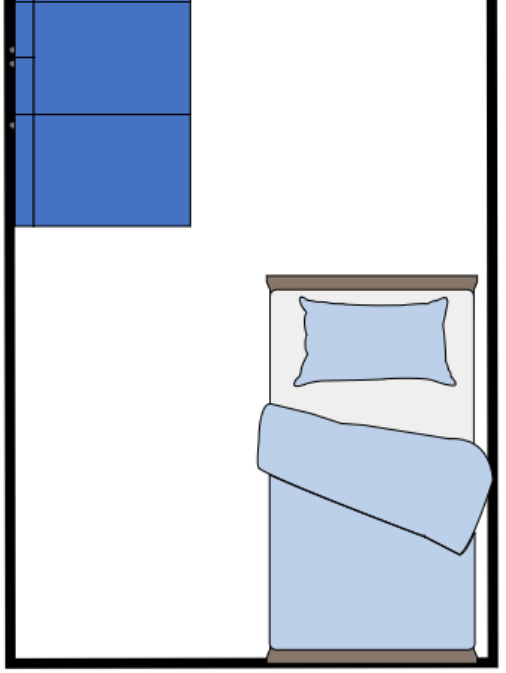
\includegraphics[width=\linewidth]{figures/Liveroom1.png}
        \caption{Guestroom evaluation environment}
        \label{fig:Liveroom1}
    \end{subfigure}
    \hfill
    \begin{subfigure}{0.35\textwidth}
        \centering
        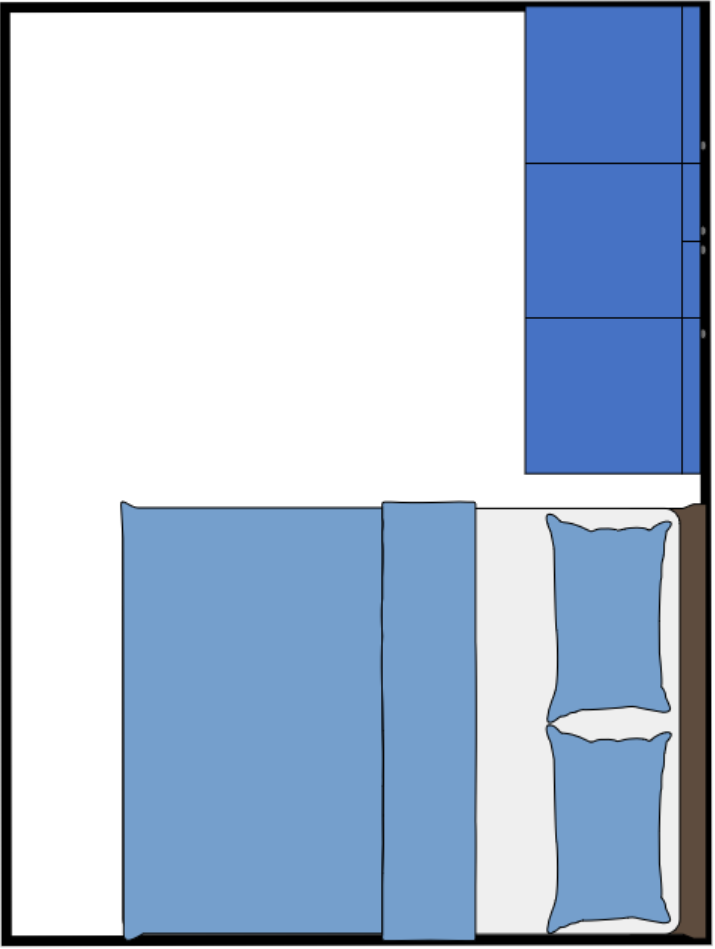
\includegraphics[width=\linewidth]{figures/Liveroom2.png}
        \caption{Bedroom evaluation environment}
        \label{fig:Liveroom2}
    \end{subfigure}
    \hfill
    \begin{subfigure}{0.45\textwidth}
        \centering
        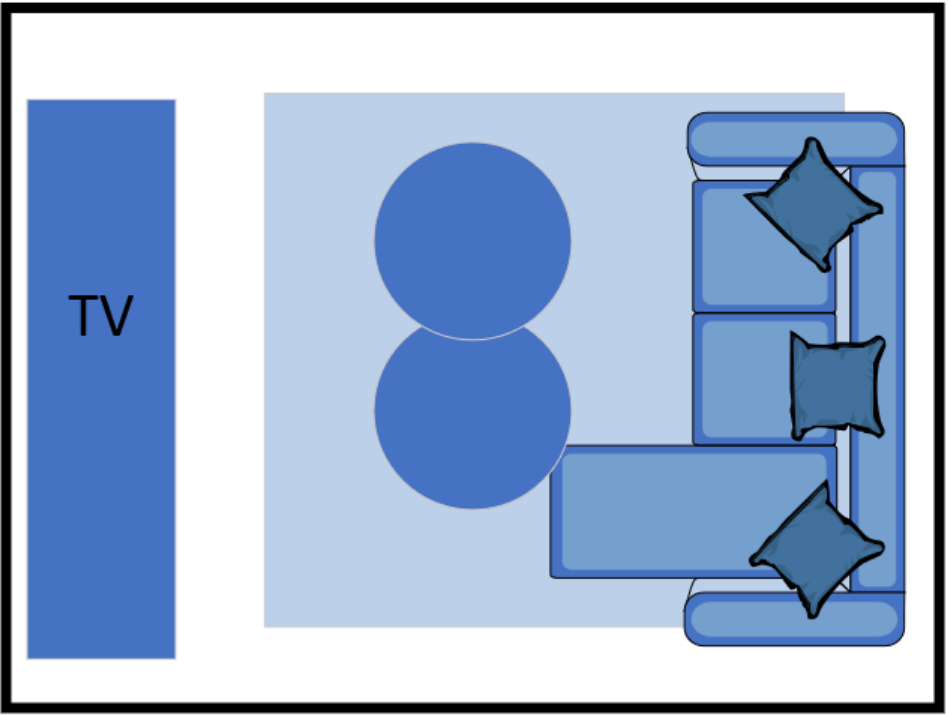
\includegraphics[width=\linewidth]{figures/Liveroom3.png}
        \caption{Living room evaluation environment}
        \label{fig:Liveroom3}
    \end{subfigure}
    
    \caption{Evaluation environments}
    \label{fig:Liveroom}
\end{figure}

For each of the evaluation environments, there was connected an additional IoT device to the same SSID as the Irobot Roomba. These devices generated traffic, simulating a real life smart home environment. the additional IoT devices are list below.

\begin{itemize}
    \item Evaluation environment 1: IPad connected
    \item Evaluation environment 2: Laptop connected
    \item Evaluation environment 3: Smart phone connected
\end{itemize}

\subsubsection{Evaluation Capturing}

All event was triggered once in each of the evaluation environments. Each event had a a 30 minute time window, were the event was triggered and finished within. The overall testing schedule is presented in the list below, were XX is the starting hour. 

\begin{itemize}
    \item Event 1: between XX:00 and XX:30
    \item Event 2: between XX:30 and XX+1:00
    \item Event 3: between XX+1:00 and XX+1:30
    \item Event 4: between XX+1:30 and XX+2:00
    \item Event 5: between XX+2:00 and XX+2:30
    \item Event 6: between XX+2:30 and XX+3:00
\end{itemize}

The event triggering order was decided by a python script, using the library \textit{random}. Scirpt logic presented in Figure \ref{fig:Sudo_code_for_event_order_randomize}. This function was executed three times, ensuring that the order of events was random and had minimum influence cross events.

\begin{figure}[H]
    \centering
    \caption{Sudo code for event order randomize}
    \label{fig:Sudo_code_for_event_order_randomize}
    \begin{lstlisting}[numbers=left]
         event_list = [scheduled_cleaning, Automated_cleaning, Application_triggered_cleaning, Application_start, Physical_triggered_cleaning, Bin_remove]
         for three rounds do:
              shuffle event_list
              print shuffeled list
    \end{lstlisting}
\end{figure}

\subsubsection{Evaluation Data Processing and Filtering}
Data processing and filtering processes are adopted from Chapter \ref{cap:Method}. Because of the added IoT devices, one additional processing step needed to be performed. To filter only based on the corresponding Irobot cloud service we needed to identify the DNS response for \textit{a2uowfjvhio0fa.iot.us-east-1.amazonaws.com}. This request occur once a day, and after a restart of the vacuum cleaner. The capturing was therefore started hour XX - 30 minutes, and the robot vacuum cleaner restarted at hour XX - 20 minutes.

Logic in Figure \ref{fig:Sudo_code_for_IP_extraction_from_DNS_response} was used to extract all IP addresses for \textit{a2uowfjvhio0fa.iot.us-east-1.amazonaws.com} in the DNS response. These addresses was added to the base filter of the extracted event files. All DNS traffic was also included in the base filter, due to their function in the detection algorithm.

\begin{figure}[H]
    \centering
    \caption{Sudo code for IP extraction from DNS response}
    \label{fig:Sudo_code_for_IP_extraction_from_DNS_response}
    \begin{lstlisting}[numbers=left]
        Fuction find_dns_response(even_capture)
          if a2uowfjvhio0fa.iot.us-east-1.amazonaws.com in event_capture
              filter = Responded Ip-addresses and dns
    \end{lstlisting}
 \end{figure}   
 
Evaluation base filter was adopted from Chapter \ref{cap:AnalysisandResults}, this filter exclude tcp-keepalive traffic, NTP, ARP, DHCP and DNS requests for TP-Link online discovery. The evaluation base filter also added two new aspects, they are listed below: 

\begin{itemize}
    \item IP-addresses equal to IP-addresses in the DNS response from \textit{a2uowfjvhio0fa.iot.us-east-1.amazonaws.com}. This excluded all traffic generated by the additional IoT device. Drawback from this implementation was that all traffic towards \textit{50315.ingest.sentry.io} and \textit{s3.amazoneaws.com} was excluded as well. The detection algorithm does not use these tcp sessions for detection, only the DNS packets. It had therefore on impact on the actual detection. 
    \item Capture file duration was 30 minutes, regardless of when the event was triggered or finished. This made the capturing files appear more as a continuous capture, and are not depend on knowledge about when the event was triggered. 
\end{itemize}

\subsection{Evaluation Results}

This subsection is presenting the data processing and rule detection results. First the event triggering sequence, followed by the DNS response IP extraction in Figure \ref{fig:Sudo_code_for_IP_extraction_from_DNS_response}, then the base filter is presented and finished by the results for event detection. 

\subsubsection{Evaluation Event Triggering Results}
Results from the randomize event order function, is presented in Table \ref{tab:evaleventoverview}. The randomization of the event triggering order, mitigates the influence cross events. 

\begin{table}[H]
\small
\centering
\caption{Evaluation event overview}
\label{tab:evaleventoverview}
\begin{tabular}{|l|l|l|l|}
\hline
\textbf{Sequence} & \textbf{Evaluation 1}          & \textbf{Evaluation 2}          & \textbf{Evaluation 3}          \\ \hline
\textbf{1}        & Automated clean                & Application start              & Remove bin                     \\ \hline
\textbf{2}        & App triggered clean            & Scheduled cleaning             & App triggered clean            \\ \hline
\textbf{3}        & Scheduled cleaning             & App triggered clean            & Phy triggered clean            \\ \hline
\textbf{4}        & Phy triggered clean            & Phy triggered clean            & Application start              \\ \hline
\textbf{5}        & Application start              & Automated clean                & Scheduled cleaning             \\ \hline
\textbf{6}        & Bin remove                     & Bin remove                     & Automated cleaning             \\ \hline
\end{tabular}
\end{table}

\subsubsection{DNS response extraction}
All evaluation environments capture files got processed by the DNS extraction algorithm. DNS responses for \textit{a2uowfjvhio0fa.iot.us-east-1.amazonaws.com}, was found in all three files, and are presented in Figure \ref{fig:Evaluation_DNSExtraction}

\begin{figure}[H]
    \centering
    
    \begin{subfigure}{0.80\textwidth}
        \centering
        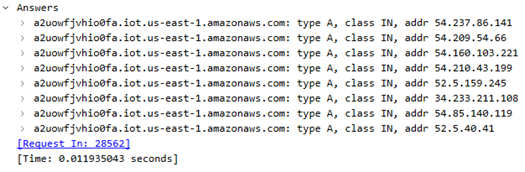
\includegraphics[width=\linewidth]{figures/Evaluation_dns_extraction 1.png}
        \caption{Guestroom DNS extraction}
        \label{fig:Evaluation_DNSextraction_1}
    \end{subfigure}
    \hfill
    \begin{subfigure}{0.80\textwidth}
        \centering
        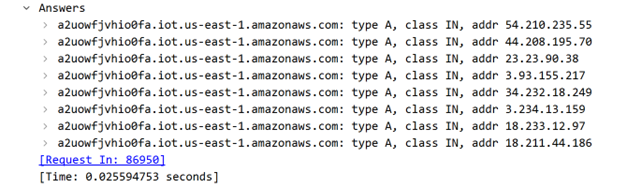
\includegraphics[width=\linewidth]{figures/Evaluation_dns_extraction 2.png}
        \caption{Bedroom DNS extraction}
        \label{fig:Evaluation_DNSextraction_2}
    \end{subfigure}
    \hfill
    \begin{subfigure}{0.80\textwidth}
        \centering
        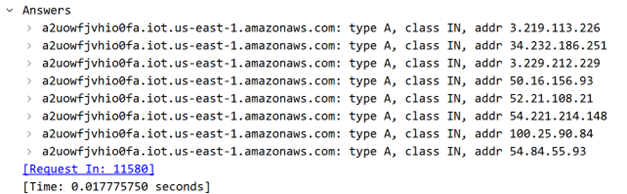
\includegraphics[width=\linewidth]{figures/Evaluation_dns_extraction 3.png}
        \caption{Living room DNS extraction}
        \label{fig:Evaluation_DNSextraction_3}
    \end{subfigure}
    
    \caption{Evaluation environment DNS extraction}
    \label{fig:Evaluation_DNSExtraction}
\end{figure}

\subsubsection{Evaluation base filter}
All evaluation filters included the same time base filter listed below. DNS responses included several IP-addresses for the corresponding Irobot cloud service, but we only included the selected one in the base filter. The selected corresponding IP address is found in Whireshark, after the Irobot Roobma receives the DNS response it establish a TCP session to one of the IP-addresses. This process is shown in Figure \ref{fig:evaluation_corresponding_cloud}


\begin{itemize}
    \item Evaluation filter: \begin{itemize}
                                \item ((frame.time >= "Apr <day>, 2023 XX:00:00") \&\& (frame.time <= "Apr <day>, 2023 XX:30:00")) AND
                                \item (frame.len > 97) AND 
                                \item  ((ip.addr == <DNS response IP>) or (dns \&\& ip.dst == 192.168.0.56))
                            \end{itemize}
    \item DNS response IP:  \begin{itemize}
                                \item Guestroom: 54.237.86.141 
                                \item Bedroom: 3.93.155.217 
                                \item Living room: 3.219.113.226 
                            \end{itemize}
\end{itemize}

\begin{figure}[H]
    \centering
    
    \begin{subfigure}{0.80\textwidth}
        \centering
        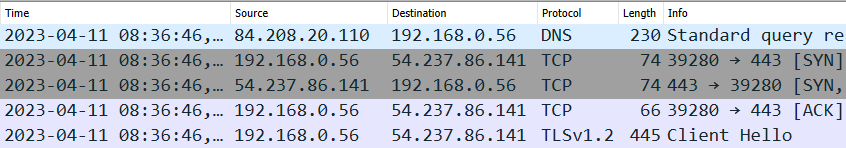
\includegraphics[width=\linewidth]{figures/Evaluation_cloud_detection1.png}
        \caption{Guestroom corresponding could detection}
        \label{fig:Evaluation_coulddetection_1}
    \end{subfigure}
    \hfill
    \begin{subfigure}{0.80\textwidth}
        \centering
        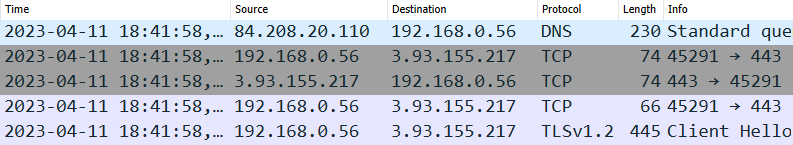
\includegraphics[width=\linewidth]{figures/Evaluation_cloud_detection2.png}
        \caption{Bedroom corresponding could detection}
        \label{fig:Evaluation_clouddetection_2}
    \end{subfigure}
    \hfill
    \begin{subfigure}{0.80\textwidth}
        \centering
        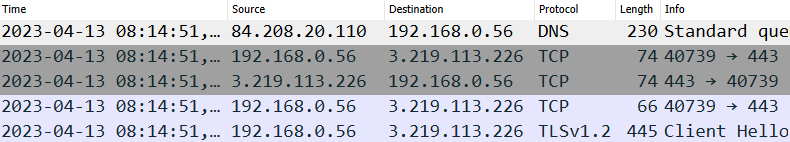
\includegraphics[width=\linewidth]{figures/Evaluation_cloud_detection3.png}
        \caption{Living room corresponding could detection}
        \label{fig:Evaluation_clouddetection_3}
    \end{subfigure}
    
    \caption{Evaluation environments corresponding could detection}
    \label{fig:evaluation_corresponding_cloud}
\end{figure}

\subsubsection{Evaluation Detection Results}
All 18 filtered capturing files was processed by the detection algorithm presented in Appendix \ref{app:DetectionAlgorithm}. No manual analysis was done to the files before hand. Detection results are presented in Table \ref{tab:Evaluation results}. Scheduled cleaning and Physical triggered cleaning is merged to one category (Sch \& Phy) in evaluation since we could not separate these based on their signatures. 

\begin{table}[H]
\small
\centering
\caption{Evaluation results}
\label{tab:Evaluation results}
\begin{tabular}{|c|c|c|c|c|c|}
\hline
\textbf{Event}        & Auto clean & App clean & Sch \& Phy & App start & Bin removed \\ \hline
\textbf{Success rate} & 100\%           & 100\%             & 100\% & 100\%             & 0\%         \\ \hline
\end{tabular}
\end{table}

The rules and detection algorithm was able to detect all events with 100\% accuracy, except bin remove. Cleaning detection resulted in True positive for all the cleaning event. If a cleaning event was detected, but not automated or application start was, it is categorized as either scheduled or physical triggered cleaning. To differentiate these tow events there should be implemented a time detection for the first "cleaning packet sequence". This timestamp can determine if it is most likely a scheduled or a physical clean en based on the start timestamp. 

Bin remove detection gave False negative for all the bin remove events. This might be because the ejection of the bin was executed without causing the Irobot Roomba to lose connection to the charging connectors. The detection algorithm also had False positive identification of bin remove event for 66\% of the automated cleaning event. The bin remove signature is therefore not usable in detection of bin removal. 


\section{Research Question 1}
\textbf{Which private information can be gathered from robot vacuum cleaner by carrying out a passive sniffing attack in a smart environment?}

It is possible to identify the presence of an Irobot vacuum cleaner inside a smart environment based on the WLAN or LAN capture itself. In WLAN eavesdropping an attacker can lookup all  MAC addresses against open source registers, here information about the manufacturer will be available. For LAN capture the presence of DNS requests to any Irobot owned domain will place a device behind the WAN address.

Other Irobot Roomba i7 events can be detected in a smart environment. Automated cleaning can be triggered by the use of location services, garage openers and door locks. All these automated triggers are indications that users are leaving the area. 

If implementations to differentiate physical triggered and scheduled cleaning are added, the detection of physical triggered cleaning will revile user activity inside the smart environment. Schedule cleaning on the other hand can give away user routines. We can assume that users usually configure scheduled cleaning when there is a high probability that there is no one at the premise. This can revile on site routines. 

For application triggered cleaning and application start it is harder to identify the actual privacy exposure. The identification of these events can revile more information if observer over longer time periods, then user patterns and behaviors can identified. If the user always trigger a cleaning event when leaving for the gym, this could be identified if collected over a longer period of time. 

As mentioned for WLAN capturing an attacker will be able to extract private information as soon as the capturing is started. This because the filter and identification of traffic is based in MAC addresses. For LAN an attacker will have to eavesdropp WAN traffic for maximum of 24 hours before the DNS request to \textit{a2uowfjvhio0fa.iot.us-east-1.amazonaws.com} is sent. 

\section{Research Question  2}
\textbf{How can the information exposed by the sniffing attack be misused by an attacker?} 

Private information exposed to an attack can be utilized to identify user behavior and routines. This could potentially revile habits of when the user is leaving the environment, and identify user presence with high confidence. This information can be used to target user environment during empty hours, or address the environment when the user is present. Such information can also be sold to other actors. 

The identification of devices can be used execute targeted attacks. Spear phishing \cite{spear_phishing} will be more effective. They can also target attack you aims to exploit known or unknown vulnerabilities for the identified devices.  

\section{Research Question  3}
\textbf{Which security measures can be implemented to limit the exposed data and decrease the risk of misuse?} 

The most efficient way to defend against the detection algorithm would be to implement a traffic sharper connected to the access point. This device could disrupt the predicted network traffic flows, pad existing packets or inject packets to break the patters. This will be an effective way to defend against this in LAN or WLAN eavesdropping. The same could be implemented on the Irobot itself, then the defence would include the wi-fi traffic as well. 

Irobot could implement random MAc addressing \cite{random_mac_bernardos2020rfc} for WLAN communication. This would allow the Irobot vacuum cleaner to use a random MAC address each time is connects to a new network, or change randomly to mislead an attacker. 

As for WAN or LAN tarffic, DNS is a easy identifier. The initial session needs to be established based on a DNS request, but consecutive changes could be transferred through the encrypted communication channel established. This could mitigate the use of DNS as detection. 



